%!TEX program = xelatex
\documentclass[UTF8,aspectratio=169,10pt,t]{ctexbeamer}

\mode<presentation> {
\usetheme{Madrid}
\setbeamertemplate{footline}[frame number] %设置页码
\setbeamercolor{page number in head/foot}{fg=blue} %设置页码颜色
\setbeamertemplate{navigation symbols}{} %去除控件
}
\usepackage{indentfirst}
\setlength{\parindent}{2em}
\usepackage{listings}
\usepackage{wrapfig}
\usepackage{graphicx}
%设置图片存放路径
\graphicspath{{figures/}}
\usepackage{multicol} %多列布局

%用户自定义区块环境
\usepackage{setspace}
\definecolor{hanblue}{rgb}{0.27, 0.42, 0.81}
\definecolor{indiagreen}{rgb}{0.07, 0.53, 0.03}
\definecolor{indianred}{rgb}{0.8, 0.36, 0.36}
\definecolor{indianyellow}{rgb}{0.89, 0.66, 0.34}
\definecolor{babypink}{rgb}{0.96, 0.76, 0.76}
\definecolor{ao(english)}{rgb}{0.0, 0.5, 0.0}
% \setbeamerfont{block title}{size=\small}
% \setbeamerfont{block body}{size=\small}
\setbeamerfont{block title}{}
\setbeamerfont{block body}{}
\newenvironment<>{blueblock}[1]{
    \setbeamercolor{block title}{fg=white,bg=hanblue}
    \begin{block}#2{#1}}{\end{block}}
\newenvironment<>{greenblock}[1]{
    \setstretch{1.3}\setbeamercolor{block title}{fg=white,bg=indiagreen}
    \begin{block}#2{#1}}{\end{block}}
\newenvironment<>{redblock}[1]{
    \setstretch{1.3}\setbeamercolor{block title}{fg=white,bg=indianred}
    \begin{block}#2{#1}}{\end{block}}
\newenvironment<>{yellowblock}[1]{
    \setstretch{1.3}\setbeamercolor{block title}{fg=white,bg=indianyellow}
    \begin{block}#2{#1}}{\end{block}}

\lstset{language=C++,
columns=flexible,
basicstyle=\footnotesize\ttfamily,                                      % 设定代码字体、大小
%numbers=left,xleftmargin=2em,framexleftmargin=2em,                   % 在左侧显示行号
%numberstyle=\color{darkgray},                                        % 设定行号格式
keywordstyle=\color{blue},                                            % 设定关键字格式
commentstyle=\color{ao(english)},                                     % 设置代码注释的格式
stringstyle=\color{brown},                                            % 设置字符串格式
%showstringspaces=false,                                              % 控制是否显示空格
%frame=lines,                                                         % 控制外框
breaklines,                                                           % 控制是否折行
postbreak=\space,                                                     % 控制折行后显示的标识字符
breakindent=5pt,                                                      % 控制折行后缩进数量
emph={size\_t,array,deque,list,map,queue,set,stack,vector,string,pair,tuple,unique\_ptr}, % 非内置类型
emphstyle={\color{teal}},
escapeinside={(*@}{@*)},
}

\title[\textit{Qt编程基础}]{Qt编程基础}

% \author
%     []
%     {}

\date{}

% \institute
%     {}


\begin{document}

\maketitle

\begin{frame}
    {目录}
    \begin{multicols*}{2}
        \tableofcontents
    \end{multicols*}
\end{frame}

\begin{frame} {前言}
    \begin{yellowblock}{学习目标}
        \begin{enumerate}
            \item 理解并掌握命名空间的使用方法;
            \item 掌握异常处理的使用方法;
            \item 理解和使用多重继承以及虚继承;
            \item 了解嵌套类和运行时类型识别的使用方法;
            \item 学会使用标准库中一些特殊工具,包括tuple类型、bitset类型以及对日期和时间的处理。
        \end{enumerate}
    \end{yellowblock}
\end{frame}

\section{Qt简介}
\begin{frame}[fragile]{13.1~Qt简介}
\vspace{-3mm}
   \begin{block}{跨平台C++图形用户界面应用程序开发框架}
  \begin{itemize}
    \item 它既可以开发GUI程序,也可用于开发非GUI程序,比如控制台工具和服务器。
    \item Qt是面向对象的框架,使用元对象编译器生成扩展代码,易于扩展,允许组件编程。
  \end{itemize}
   \end{block}
\vspace{-2.3mm}
    \begin{columns}[T]
        \column{0.5\textwidth}
        \pause \centering 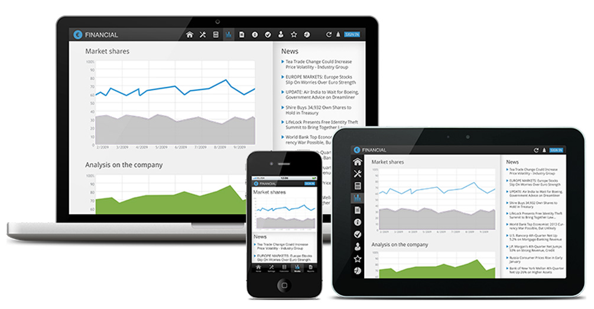
\includegraphics[width=0.66\textwidth]{fig/fig1} \vspace{-2.3mm}
   \begin{block}{跨平台}
 桌面OS:Windows, Linux, Mac; 移动OS:iOS, Android,WP; 嵌入式OS: QNX,VxWorks 
  \end{block}
  \column{0.45\textwidth}
   \pause
 \centering 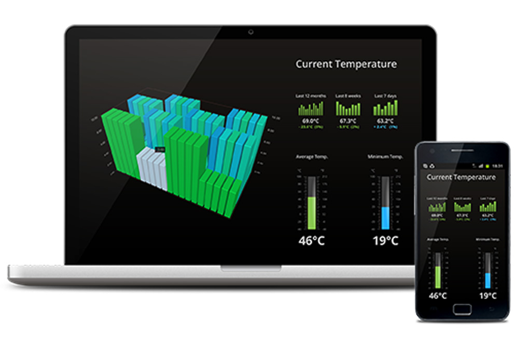
\includegraphics[width=0.58\textwidth]{fig/fig2}\vspace{-2.3mm}
   \begin{block}{集成开发平台}
 Design, Code, Debug \& Deploy Quickly\\
 ~~
  \end{block}
  \end{columns}
  \vspace{2mm}
\pause
\noindent \parbox{\textwidth}{应用:WPS、Skype、豆瓣电台、虾米音乐、暴雪的战网客户端、VirtualBox、Opera、咪咕音乐、\\Google地图、Adobe Photoshop Album}
\end{frame}


\end{document} 